% COMP0228 Coursework 1 -- evidence-based working draft, 25 October 2026.
% OVERLEAF: create a blank project, paste this entire file into main.tex,
% select pdfLaTeX, and compile. No figures, .bib files or shell escape needed.
% IEEEtran controls the typography and margins; do not shrink these to fit.
% EDIT FIRST: replace the four author placeholders below.
% BEFORE SUBMISSION: every member must review and understand the claims;
% check the Moodle rubric and contribution form separately. This is a draft,
% not a claim that the group has already completed that review.
%
% STRUCTURE / SECTION OWNERSHIP (these comments do not appear in the PDF):
% I   Why: motivation, prior work, questions, contributions.
% II  What: implemented system, codes and two extensions.
% III How tested: datasets, controls, metrics, uncertainty, verification.
% IV  What happened: results, ordered by the questions in Section I.
% V   What it means: trade-offs, scope and threats to validity.
% VI  Answer: concise conclusions supported by Sections IV--V.
% Do not repeat implementation detail in Results or add new results in VI.
%
% LOCAL EVIDENCE (paths relative to the optical_link project):
% data/analysis/receiver_layers_2026-10-24/{manifest,frozen_config}.json
% data/analysis/receiver_layers_2026-10-24/results/{summary,all_results}.json
% data/analysis/coding_experiments_2026-10-24/{config,summary,paired_outcomes}.json
% data/analysis/coding_experiments_2026-10-24/physical_noise.json
% data/analysis/coding_experiments_2026-10-24/independent_audit.json
% All plotted values are embedded from these saved outputs. If experiments
% change, update the numbers, plots, abstract and conclusion together.
% Analysis data is included in Git; silent recordings are optional
% downloads from the data-v1.1.0 release. See data/recordings_manifest.json.

\documentclass[conference,a4paper]{IEEEtran}
\usepackage[T1]{fontenc}
\usepackage{amsmath,amssymb}
\usepackage{booktabs,array}
\usepackage{cite}
\usepackage{xcolor}
\usepackage{tikz}
\usetikzlibrary{arrows.meta,positioning}
\usepackage{pgfplots}
\usepgfplotslibrary{groupplots}
\pgfplotsset{compat=1.18}
\usepackage[hidelinks]{hyperref}
\urlstyle{same}

\newcommand{\GroupAuthors}{Student 1, Student 2, Student 3, and Student 4}
\newcommand{\BER}{\operatorname{BER}}
\definecolor{codeblue}{RGB}{0,114,178}
\definecolor{codeorange}{RGB}{213,94,0}
\definecolor{codegreen}{RGB}{0,135,104}
\definecolor{codepurple}{RGB}{160,80,145}
\pgfplotsset{
  paperaxis/.style={
    font=\footnotesize, tick label style={font=\scriptsize},
    label style={font=\footnotesize}, title style={font=\footnotesize},
    axis line style={black!65}, tick style={black!65},
    grid=major, grid style={black!10},
    legend style={font=\scriptsize,draw=none},
    scaled ticks=false, unbounded coords=jump
  },
  nocode/.style={black!75,mark=o,mark size=1.3pt,solid},
  repthree/.style={codeorange,mark=square*,mark size=1.3pt,dashed},
  repfive/.style={codepurple,mark=triangle*,mark size=1.5pt,dashdotted},
  hamming/.style={codeblue,mark=diamond*,mark size=1.5pt,solid},
  reedsolomon/.style={codegreen,mark=*,mark size=1.3pt,densely dashed}
}

\title{Error Structure, Coding and Receiver Design\\
for a Screen-to-Camera Optical Link}
\author{\IEEEauthorblockN{\GroupAuthors}
\IEEEauthorblockA{University College London\\
COMP0228: Compression, Sampling and Data Analysis --- Coursework 1}}

\begin{document}
\maketitle

\begin{abstract}
Error correction depends on how a channel corrupts data, as well as on the
amount of redundancy transmitted. We investigate this relationship using a
flashing display, a phone camera and physical light interference. The system
compares uncoded transmission, two repetition levels, Hamming coding and
Reed--Solomon coding. Thirty recorded packets exhibit 180 baseline channel
errors, all changing a zero to a one, including consecutive error runs of up
to eight bits. Two extensions address different stages of this failure:
reference-based and spatial receiver preprocessing, and bit interleaving.
Preprocessing increases exact, checksum-valid recovery from 8 to 30 packets
on the recorded dataset; eight packets informed parameter selection and the
remaining recordings are not a blind test. Separately, 480,000 synthetic
decoding evaluations isolate noise structure and transmission cost. Under
one burst-flip condition, interleaving raises Hamming packet success from
40.25\% to 66.70\%, but lowers Reed--Solomon success from 78.05\% to 53.90\%.
These results support matching receiver processing and coding to the error
mechanism. They do not establish universal reliability: physical sampling
is limited, and the simulations assume successful synchronisation and
header reception.
\end{abstract}

\begin{IEEEkeywords}
optical communication, error correction, burst noise, interleaving,
experimental evaluation
\end{IEEEkeywords}

\section{Introduction}
\label{sec:intro}
Reliable communication requires a receiver to recover information from a
distorted physical signal. Extra parity can repair some errors, but it also
lengthens transmission. If interference corrupts adjacent bits together,
adding redundancy without considering its arrangement can provide little
benefit. A useful evaluation must therefore ask both whether a message is
recovered and how much channel time that recovery consumes.

Classical Hamming codes protect small binary blocks, whereas
Reed--Solomon codes operate on larger symbols~\cite{hamming,reedsolomon}.
Their different correction units make error structure consequential.
Two-state channel models provide a way to study temporal
clustering~\cite{gilbert}. Optical receivers also face illumination offsets;
Pham \emph{et al.} demonstrate ambient-light rejection in a photodiode
receiver~\cite{pham}. Our camera implementation uses image regions rather
than that analogue circuit, and does not inherit its performance claims.

We study a deliberately slow screen-to-camera link that makes the full
chain observable: message, coded bits, physical flashes, measured
brightness, decoded bits and validated payload. The central question is:
\emph{How should coding and receiver processing be matched to observed
optical errors, while accounting for transmission cost?} Three subsidiary
questions organise the evaluation:
\begin{enumerate}
  \item What error directions and temporal patterns occur in the physical
  channel, and how do the baseline codes behave?
  \item Can illumination compensation and spatial aggregation improve
  decoding of the same recordings?
  \item When does interleaving improve reliability and useful throughput,
  and when does it harm a code?
\end{enumerate}

The contributions are an auditable physical link with five coding
configurations; a comparison that separates receiver processing from
coding; and controlled experiments exposing both beneficial and harmful
effects of interleaving. These are implementation and experimental
contributions, not claims of new coding theory. Section~\ref{sec:system}
defines the system, Section~\ref{sec:design} the evaluation, and
Sections~\ref{sec:results}--\ref{sec:discussion} the findings and their scope.

\section{System and Methods}
\label{sec:system}
\subsection{Physical Channel and Packet Format}
An ESP32-S3 drives a LAFVIN display with an ST7796S controller using
LovyanGFX~\cite{lovyangfx}. A central patch displays white for one and black
for zero, with a nominal bit duration $T_b=0.2$~s. An iPhone records the
screen. Moving a light across the display introduces physical illumination
interference; the transmitted bit sequence itself is unchanged.
Figure~\ref{fig:system} separates the receiver from evaluation against the
sent-message log.

Each packet contains an eight-bit dark guard, a 32-bit public preamble, a
48-bit header, a coded body, and a final eight-bit guard. The header carries
version, coding mode, payload length and sequence number, protected by a
16-bit cyclic redundancy check (CRC). The body contains the payload and a
second 16-bit CRC covering the four metadata bytes and payload, followed
by the chosen error-correcting encoding. Both checks use polynomial
\texttt{0x1021} with initial value \texttt{0xFFFF}. Thus fixed framing costs
96 bit slots in addition to the coded body. The CRC detects errors; it
does not itself correct them.

\begin{figure}[t]
\centering
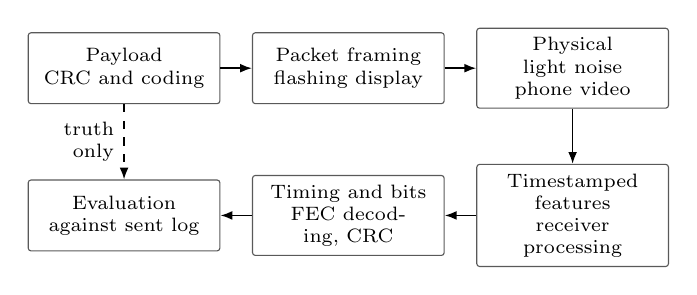
\begin{tikzpicture}[
  node distance=4mm and 4mm,
  box/.style={draw=black!65,rounded corners=1pt,align=center,
              text width=22mm,minimum height=9mm,font=\scriptsize},
  flow/.style={-{Latex[length=1.5mm]},semithick}]
  \node[box] (msg) {Payload\\CRC and coding};
  \node[box,right=of msg] (tx) {Packet framing\\flashing display};
  \node[box,right=of tx] (cam) {Physical light noise\\phone video};
  \node[box,below=7mm of cam] (front) {Timestamped features\\receiver processing};
  \node[box,left=of front] (dec) {Timing and bits\\FEC decoding, CRC};
  \node[box,left=of dec] (eval) {Evaluation\\against sent log};
  \draw[flow] (msg)--(tx);
  \draw[flow] (tx)--(cam);
  \draw[flow] (cam)--(front);
  \draw[flow] (front)--(dec);
  \draw[flow] (dec)--(eval);
  \draw[flow,dashed] (msg)--node[left,font=\scriptsize,align=right]
       {truth\\only} (eval);
\end{tikzpicture}
\caption{The optical link and evaluation boundary. Sent payloads enter the
evaluator only, not the receiver. FEC denotes forward error correction.}
\label{fig:system}
\end{figure}

\subsection{Baseline Receiver and Coding}
Brightness is extracted from a fixed image region using grayscale frame
values and actual video timestamps. The public preamble supplies the
optical start time, fitted bit period and dark/bright calibration levels.
The decision threshold is the midpoint of those levels. Each bit uses the
median brightness in the middle half of its fitted time slot, avoiding
transition edges. Missing samples and invalid headers produce failures
rather than inferred replacement bits. Acquisition initially uses
trace-wide brightness percentiles; subsequent level calibration uses the
preamble. Neither stage sees the expected payload or transmission time.

Repetition sends each bit three or five times and uses majority voting.
Hamming$(7,4)$ uses even parity and syndrome decoding to correct one error
per seven-bit word; multiple errors can cause miscorrection. The
independently researched approach is a shortened Reed--Solomon code over
$\mathrm{GF}(256)$ with four parity bytes, correcting up to two erroneous
byte symbols per body. We integrate the credited \texttt{reedsolo}~1.7.0
library~\cite{reedsolo}; the decoder is not an original implementation.
Table~\ref{tab:codes} makes the cost of redundancy explicit.

\begin{table}[t]
\caption{Coding cost for a nine-byte payload. The uncoded body includes
two CRC bytes. Airtime includes all 96 framing slots at 0.2~s/bit.}
\label{tab:codes}
\centering
\footnotesize
\begin{tabular}{@{}lrrr@{}}
\toprule
Code & Body bits & Airtime (s) & Clean goodput (bit/s)\\
\midrule
Uncoded & 88 & 36.8 & 1.957\\
Repetition $\times3$ & 264 & 72.0 & 1.000\\
Repetition $\times5$ & 440 & 107.2 & 0.672\\
Hamming$(7,4)$ & 154 & 50.0 & 1.440\\
Reed--Solomon & 120 & 43.2 & 1.667\\
\bottomrule
\end{tabular}
\end{table}

\subsection{Extension 1: Receiver Preprocessing}
Two complementary operations target positive illumination changes.
\emph{Reference compensation} measures four non-flashing regions. For
reference brightness $r_j(t)$ and its preamble median $c_j$, the estimated
shared change is
\begin{equation}
  o(t)=\operatorname{median}_{j=1,\ldots,4}\{r_j(t)-c_j\}.
\end{equation}
Subtracting $\alpha o(t)$ from patch brightness suppresses changes shared
by the patch and its surroundings.

\emph{Spatial aggregation} divides the patch into $5\times5$ tiles. Each
tile is normalised using its own preamble dark and bright medians. Tiles
with contrast below 20 grayscale units are discarded; at least 13 of the
25 tiles must remain usable. The signal is the lower quartile of the
normalised tile values, rescaled before thresholding. A local bright
reflection can then affect some tiles without controlling the aggregate.
This choice targets positive glare and is not a general solution to
arbitrary occlusion.

The combined method subtracts the reference offset from each tile before
normalisation and aggregation. All variants share the original receiver's
preamble acquisition and clock. A larger-patch mean control separates
changes in image support from changes in processing. The five variants
are therefore original region mean, larger-patch mean, reference only,
spatial only and combined. No variant uses the known message to tune a
threshold during reception.

\subsection{Extension 2: Bit Interleaving}
An eight-row ragged matrix is filled row-wise with the coded body and read
column-wise, omitting unused cells. The receiver reverses this permutation
before decoding. Interleaving adds no transmitted bits but buffers one
coded body. It is evaluated in simulation, not in new physical
transmissions. Its purpose is to redistribute adjacent channel errors
across correction units; for byte-oriented Reed--Solomon, the same
operation may instead spread damage into too many byte symbols. The
experiment therefore includes harms as well as rescues.

\section{Experimental Design}
\label{sec:design}
\subsection{Physical Recordings and Paired Receiver Evaluation}
The evidence comprises 30 packets in 14 videos: eight development packets
and two later batches of 11 packets each. Four packets are clean controls
and 26 contain physical interference. Each coding configuration appears
six times, but payloads, clean-control allocation and interference are not
balanced across codes. These recordings establish channel behaviour and
support paired reprocessing; they are not a controlled ranking of codes.

Every receiver variant processes the same stored frames with fixed,
video-specific geometry. Reference gains $\{0.5,1,1.5\}$ and spatial
quantiles $\{0.25,0.5\}$ were compared on the eight development packets.
Selection minimised clean-control failures first, then all development
failures, missing outputs and channel bit errors. Selected component
settings were $\alpha=1$ and quantile $0.25$; their combination introduced
no further search. Source and geometry hashes were frozen before scoring
the new receiver variants on the later 22 packets. However, those videos
and their baseline results had already been inspected: this is a
retrospective evaluation, not a pristine blind holdout.

\subsection{Controlled Coding and Interleaving Experiments}
Simulations use the actual packet encoders and decoders with nine uniformly
random payload bytes. They assume correct acquisition and header reception,
apply noise only to the coded body, and still charge full framing airtime.
Three models separate error mechanisms:
\begin{enumerate}
  \item \emph{Independent flips}: each wire bit flips with probability $p$.
  \item \emph{Burst flips}: a stationary two-state Markov process flips
  every bit in the bad state.
  \item \emph{Glare bursts}: the same process forces bad-state bits to one;
  already-bright bits are unchanged.
\end{enumerate}
For bad-state occupancy $\rho$ and mean bad-run length $L$ slots, transitions
are
\begin{equation}
  P(B\!\to\!G)=\frac{1}{L},\qquad
  P(G\!\to\!B)=\frac{\rho}{(1-\rho)L}.
  \label{eq:markov}
\end{equation}
Trials start in stationarity and are independent across trial indices.
This is a deliberately simplified Gilbert-style model~\cite{gilbert}, not
a fitted optical channel. For flips, occupancy equals expected bit-error
probability; for glare it does not, because only zeros can be corrupted.

The rate sweep uses $\{0,0.01,0.025,0.05,0.10,0.20\}$ with $L=8$. A further
burst-duration sweep uses $L\in\{2,4,8,16\}$ at $\rho=0.05$. Removing
duplicated conditions leaves 24 noise settings, each evaluated with five
codes and depths one and eight. At 2,000 trials per condition this gives
480,000 decoding evaluations. Settings and seed 20261024 were fixed before
the main run. Codes and depths share payloads and the same noise-process
prefix within each trial; longer transmissions encounter more channel
slots. The total is not a count of independent physical observations.

\subsection{Metrics, Uncertainty and Verification}
Let $b_i$ be the payload length in bits, $n_i$ the coded-body length, $e_i$
the pre-correction body errors, and $s_i=1$ only when the payload is exact
\emph{and} its CRC passes. We report
\begin{equation}
  \BER_{\mathrm{ch}}=\frac{\sum_i e_i}{\sum_i n_i},\qquad
  \widehat P_s=\frac{1}{N}\sum_{i=1}^{N}s_i,
\end{equation}
and verified payload goodput
\begin{equation}
  G=\frac{\sum_i b_i s_i}{\sum_i T_b(96+n_i)}.
  \label{eq:goodput}
\end{equation}
Failed packets contribute their full airtime and zero delivered bits.
This is on-channel goodput, excluding file transfer, operator setup and
offline processing time. Payload BER is conditional on a decoder output;
rejections remain explicit failures. A damaged or absent output is never
silently treated as error-free.

Simulation packet probabilities have 95\% Wilson intervals~\cite{wilson}.
At fixed payload and duration, multiplying these limits by the offered
payload rate gives goodput intervals. Comparisons also count paired
rescues and harms, rather than treating paired outcomes as independent.
Physical counts are descriptive because packets share videos and manually
created interference. Bursty bits are not independent statistical samples.

Seventy-two software tests pass. The saved audit verifies all 480,000 trial
records and recomputes their summaries, checks 30 zero-noise configurations,
compares 60 independent-flip configurations with analytic predictions, and
replays 720 decodes. Source/data hashes, frozen receiver settings and the
main notebook link reported results to stored evidence. These checks
support implementation correctness; they do not remove experimental bias.

\begin{figure}[t]
\centering
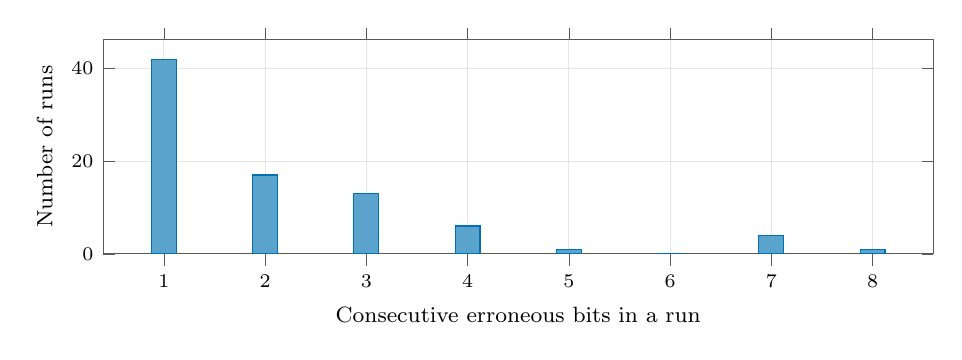
\begin{tikzpicture}
\begin{axis}[paperaxis,width=\columnwidth,height=43mm,
  ybar,bar width=9pt,xmin=0.4,xmax=8.6,ymin=0,
  xtick={1,2,3,4,5,6,7,8},
  xlabel={Consecutive erroneous bits in a run},ylabel={Number of runs}]
\addplot[fill=codeblue!65,draw=codeblue] coordinates {(1,42) (2,17) (3,13) (4,6) (5,1) (6,0) (7,4) (8,1)};
\end{axis}
\end{tikzpicture}
\caption{Observed baseline error runs, pooled over the 30 physical packets
without joining packet boundaries. All 180 errors are $0\to1$.
Error-run length is not the duration of a light sweep: intervening ones
can hide a continuous bright disturbance.}
\label{fig:runs}
\end{figure}

\begin{figure*}[t]
\centering
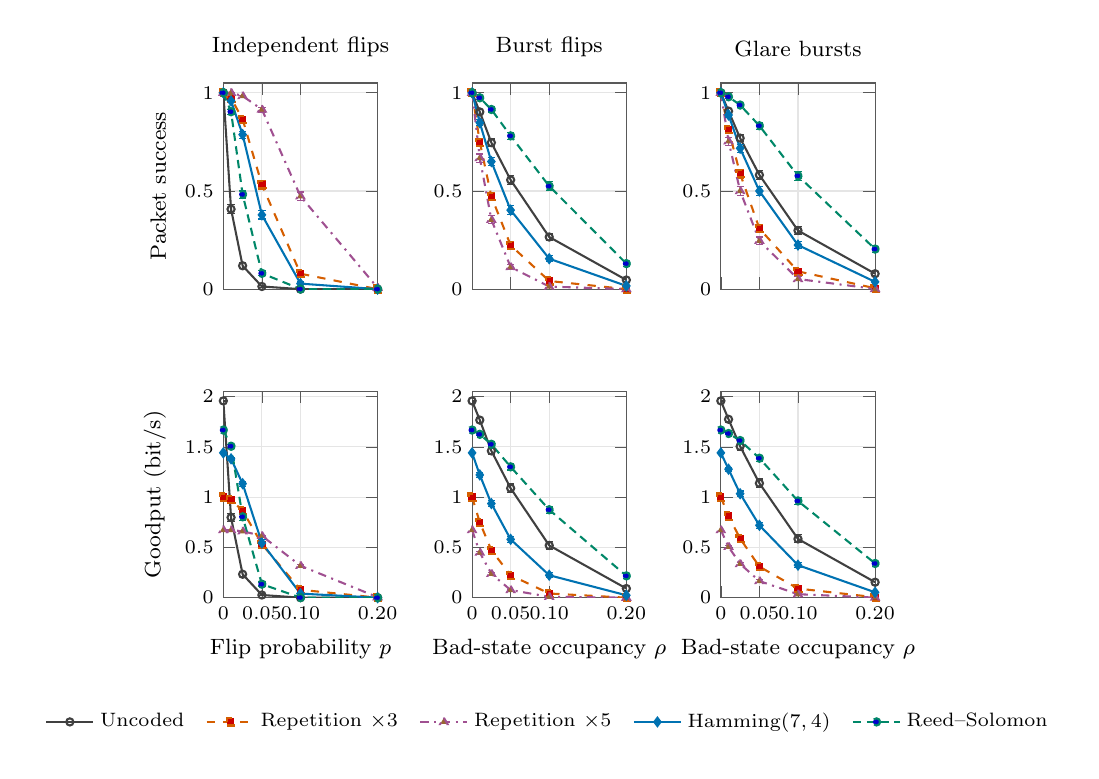
\begin{tikzpicture}
\begin{groupplot}[
  paperaxis,
  group style={group size=3 by 2,horizontal sep=12mm,vertical sep=13mm},
  width=0.292\textwidth,height=42mm,
  xmin=0,xmax=0.20,xtick={0,0.05,0.10,0.20},
  xticklabels={0,0.05,0.10,0.20},
  every axis plot/.append style={line width=0.75pt},
  error bars/y dir=both,error bars/y explicit,
  error bars/error bar style={line width=0.4pt},
  error bars/error mark options={rotate=90,mark size=1.3pt}
]
\nextgroupplot[ymin=0,ymax=1.05,title={Independent flips},xticklabels={,, ,},ylabel={Packet success},legend to name=codelegend,legend columns=5,legend style={font=\scriptsize,draw=none,/tikz/every even column/.append style={column sep=2mm}}]
\addplot+[nocode] coordinates {
(0,1) += (0,0) -= (0,0.0019170473)
(0.01,0.4075) += (0,0.021692218) -= (0,0.021337564)
(0.025,0.119) += (0,0.014925986) -= (0,0.013465196)
(0.05,0.0135) += (0,0.006070793) -= (0,0.004205506)
(0.1,0) += (0,0.0019170473) -= (0,0)
(0.2,0) += (0,0.0019170473) -= (0,0)
};
\addlegendentry{Uncoded}
\addplot+[repthree] coordinates {
(0,1) += (0,0) -= (0,0.0019170473)
(0.01,0.9725) += (0,0.0063115018) -= (0,0.0081231115)
(0.025,0.8655) += (0,0.014254384) -= (0,0.015655745)
(0.05,0.532) += (0,0.021785909) -= (0,0.0219086)
(0.1,0.0785) += (0,0.012611756) -= (0,0.010995685)
(0.2,0) += (0,0.0019170473) -= (0,0)
};
\addlegendentry{Repetition $\times3$}
\addplot+[repfive] coordinates {
(0,1) += (0,0) -= (0,0.0019170473)
(0.01,1) += (0,0) -= (0,0.0019170473)
(0.025,0.9835) += (0,0.0047271764) -= (0,0.0065809611)
(0.05,0.915) += (0,0.011440899) -= (0,0.013032048)
(0.1,0.473) += (0,0.021911929) -= (0,0.021808408)
(0.2,0.007) += (0,0.0047158626) -= (0,0.0028256539)
};
\addlegendentry{Repetition $\times5$}
\addplot+[hamming] coordinates {
(0,1) += (0,0) -= (0,0.0019170473)
(0.01,0.9585) += (0,0.0078976168) -= (0,0.0096555492)
(0.025,0.787) += (0,0.017384669) -= (0,0.018485054)
(0.05,0.378) += (0,0.021465535) -= (0,0.020997776)
(0.1,0.028) += (0,0.0081844827) -= (0,0.0063747901)
(0.2,0) += (0,0.0019170473) -= (0,0)
};
\addlegendentry{Hamming$(7,4)$}
\addplot+[reedsolomon] coordinates {
(0,1) += (0,0) -= (0,0.0019170473)
(0.01,0.9035) += (0,0.012177973) -= (0,0.01372503)
(0.025,0.4825) += (0,0.02191221) -= (0,0.021845114)
(0.05,0.0805) += (0,0.012743468) -= (0,0.011135066)
(0.1,0.0005) += (0,0.0023268625) -= (0,0.00041173227)
(0.2,0) += (0,0.0019170473) -= (0,0)
};
\addlegendentry{Reed--Solomon}
\nextgroupplot[ymin=0,ymax=1.05,title={Burst flips},xticklabels={,, ,}]
\addplot+[nocode] coordinates {
(0,1) += (0,0) -= (0,0.0019170473)
(0.01,0.9025) += (0,0.01223929) -= (0,0.013782513)
(0.025,0.746) += (0,0.018593353) -= (0,0.01953654)
(0.05,0.556) += (0,0.021647219) -= (0,0.021861929)
(0.1,0.2655) += (0,0.019789791) -= (0,0.018890696)
(0.2,0.0465) += (0,0.010129693) -= (0,0.0083909315)
};
\addplot+[repthree] coordinates {
(0,1) += (0,0) -= (0,0.0019170473)
(0.01,0.7485) += (0,0.018526424) -= (0,0.019479196)
(0.025,0.472) += (0,0.021911439) -= (0,0.021804084)
(0.05,0.223) += (0,0.018764252) -= (0,0.017702208)
(0.1,0.0415) += (0,0.0096555492) -= (0,0.0078976168)
(0.2,0) += (0,0.0019170473) -= (0,0)
};
\addplot+[repfive] coordinates {
(0,1) += (0,0) -= (0,0.0019170473)
(0.01,0.668) += (0,0.02029974) -= (0,0.020943868)
(0.025,0.3535) += (0,0.021213992) -= (0,0.020652297)
(0.05,0.1125) += (0,0.014597711) -= (0,0.013112)
(0.1,0.013) += (0,0.0059803085) -= (0,0.0041131045)
(0.2,0) += (0,0.0019170473) -= (0,0)
};
\addplot+[hamming] coordinates {
(0,1) += (0,0) -= (0,0.0019170473)
(0.01,0.8475) += (0,0.015088513) -= (0,0.016420861)
(0.025,0.6495) += (0,0.020605923) -= (0,0.021179121)
(0.05,0.4025) += (0,0.021659519) -= (0,0.021285694)
(0.1,0.155) += (0,0.016520848) -= (0,0.015198086)
(0.2,0.0165) += (0,0.0065809611) -= (0,0.0047271764)
};
\addplot+[reedsolomon] coordinates {
(0,1) += (0,0) -= (0,0.0019170473)
(0.01,0.9745) += (0,0.0060520842) -= (0,0.007871362)
(0.025,0.915) += (0,0.011440899) -= (0,0.013032048)
(0.05,0.7805) += (0,0.017592829) -= (0,0.018668292)
(0.1,0.5245) += (0,0.021818835) -= (0,0.02191277)
(0.2,0.13) += (0,0.015451124) -= (0,0.014032509)
};
\nextgroupplot[ymin=0,ymax=1.05,title={Glare bursts},xticklabels={,, ,}]
\addplot+[nocode] coordinates {
(0,1) += (0,0) -= (0,0.0019170473)
(0.01,0.9065) += (0,0.011991464) -= (0,0.013550023)
(0.025,0.769) += (0,0.017945308) -= (0,0.01897668)
(0.05,0.5815) += (0,0.021443592) -= (0,0.021756071)
(0.1,0.2985) += (0,0.020425611) -= (0,0.019653041)
(0.2,0.0785) += (0,0.012611756) -= (0,0.010995685)
};
\addplot+[repthree] coordinates {
(0,1) += (0,0) -= (0,0.0019170473)
(0.01,0.8115) += (0,0.016537688) -= (0,0.017732008)
(0.025,0.5875) += (0,0.021387132) -= (0,0.021722615)
(0.05,0.3085) += (0,0.020593191) -= (0,0.019858962)
(0.1,0.0905) += (0,0.013371053) -= (0,0.011800991)
(0.2,0.0045) += (0,0.0040305132) -= (0,0.0021307194)
};
\addplot+[repfive] coordinates {
(0,1) += (0,0) -= (0,0.0019170473)
(0.01,0.753) += (0,0.01840384) -= (0,0.019373866)
(0.025,0.5) += (0,0.021892049) -= (0,0.021892049)
(0.05,0.246) += (0,0.019350087) -= (0,0.018376227)
(0.1,0.0515) += (0,0.010574871) -= (0,0.0088552799)
(0.2,0.001) += (0,0.0026389343) -= (0,0.00072572108)
};
\addplot+[hamming] coordinates {
(0,1) += (0,0) -= (0,0.0019170473)
(0.01,0.887) += (0,0.013139672) -= (0,0.014623467)
(0.025,0.7175) += (0,0.019299719) -= (0,0.020133635)
(0.05,0.4995) += (0,0.021892997) -= (0,0.02189108)
(0.1,0.2245) += (0,0.018804809) -= (0,0.017748516)
(0.2,0.037) += (0,0.009199881) -= (0,0.0074246952)
};
\addplot+[reedsolomon] coordinates {
(0,1) += (0,0) -= (0,0.0019170473)
(0.01,0.9795) += (0,0.0053528411) -= (0,0.0071912895)
(0.025,0.9375) += (0,0.0097928684) -= (0,0.011470285)
(0.05,0.832) += (0,0.015745307) -= (0,0.017018226)
(0.1,0.577) += (0,0.021483787) -= (0,0.021779012)
(0.2,0.204) += (0,0.018220202) -= (0,0.01708531)
};
\nextgroupplot[ymin=0,ymax=2.05,xlabel={Flip probability $p$},ylabel={Goodput (bit/s)}]
\addplot+[nocode] coordinates {
(0,1.9565217) += (0,0) -= (0,0.0037507447)
(0.01,0.79728261) += (0,0.042441296) -= (0,0.041747408)
(0.025,0.23282609) += (0,0.029203016) -= (0,0.026344948)
(0.05,0.026413043) += (0,0.011877638) -= (0,0.0082281639)
(0.1,0) += (0,0.0037507447) -= (0,0)
(0.2,0) += (0,0.0037507447) -= (0,0)
};
\addplot+[repthree] coordinates {
(0,1) += (0,0) -= (0,0.0019170473)
(0.01,0.9725) += (0,0.0063115018) -= (0,0.0081231115)
(0.025,0.8655) += (0,0.014254384) -= (0,0.015655745)
(0.05,0.532) += (0,0.021785909) -= (0,0.0219086)
(0.1,0.0785) += (0,0.012611756) -= (0,0.010995685)
(0.2,0) += (0,0.0019170473) -= (0,0)
};
\addplot+[repfive] coordinates {
(0,0.67164179) += (0,0) -= (0,0.0012875691)
(0.01,0.67164179) += (0,0) -= (0,0.0012875691)
(0.025,0.6605597) += (0,0.0031749692) -= (0,0.0044200485)
(0.05,0.61455224) += (0,0.007684186) -= (0,0.0087528683)
(0.1,0.31768657) += (0,0.014716967) -= (0,0.014647438)
(0.2,0.0047014925) += (0,0.0031673704) -= (0,0.0018978273)
};
\addplot+[hamming] coordinates {
(0,1.44) += (0,0) -= (0,0.0027605481)
(0.01,1.38024) += (0,0.011372568) -= (0,0.013903991)
(0.025,1.13328) += (0,0.025033924) -= (0,0.026618478)
(0.05,0.54432) += (0,0.030910371) -= (0,0.030236797)
(0.1,0.04032) += (0,0.011785655) -= (0,0.0091796977)
(0.2,0) += (0,0.0027605481) -= (0,0)
};
\addplot+[reedsolomon] coordinates {
(0,1.6666667) += (0,0) -= (0,0.0031950788)
(0.01,1.5058333) += (0,0.020296621) -= (0,0.02287505)
(0.025,0.80416667) += (0,0.036520351) -= (0,0.036408523)
(0.05,0.13416667) += (0,0.021239114) -= (0,0.018558443)
(0.1,0.00083333333) += (0,0.0038781042) -= (0,0.00068622045)
(0.2,0) += (0,0.0031950788) -= (0,0)
};
\nextgroupplot[ymin=0,ymax=2.05,xlabel={Bad-state occupancy $\rho$}]
\addplot+[nocode] coordinates {
(0,1.9565217) += (0,0) -= (0,0.0037507447)
(0.01,1.7657609) += (0,0.023946437) -= (0,0.026965787)
(0.025,1.4595652) += (0,0.036378299) -= (0,0.038223666)
(0.05,1.0878261) += (0,0.042353255) -= (0,0.042773338)
(0.1,0.51945652) += (0,0.038719156) -= (0,0.036960056)
(0.2,0.090978261) += (0,0.019818965) -= (0,0.01641704)
};
\addplot+[repthree] coordinates {
(0,1) += (0,0) -= (0,0.0019170473)
(0.01,0.7485) += (0,0.018526424) -= (0,0.019479196)
(0.025,0.472) += (0,0.021911439) -= (0,0.021804084)
(0.05,0.223) += (0,0.018764252) -= (0,0.017702208)
(0.1,0.0415) += (0,0.0096555492) -= (0,0.0078976168)
(0.2,0) += (0,0.0019170473) -= (0,0)
};
\addplot+[repfive] coordinates {
(0,0.67164179) += (0,0) -= (0,0.0012875691)
(0.01,0.44865672) += (0,0.013634154) -= (0,0.014066777)
(0.025,0.23742537) += (0,0.014248204) -= (0,0.013870946)
(0.05,0.075559701) += (0,0.0098044331) -= (0,0.008806567)
(0.1,0.0087313433) += (0,0.0040166251) -= (0,0.0027625328)
(0.2,0) += (0,0.0012875691) -= (0,0)
};
\addplot+[hamming] coordinates {
(0,1.44) += (0,0) -= (0,0.0027605481)
(0.01,1.2204) += (0,0.021727459) -= (0,0.02364604)
(0.025,0.93528) += (0,0.02967253) -= (0,0.030497934)
(0.05,0.5796) += (0,0.031189707) -= (0,0.0306514)
(0.1,0.2232) += (0,0.023790022) -= (0,0.021885243)
(0.2,0.02376) += (0,0.009476584) -= (0,0.006807134)
};
\addplot+[reedsolomon] coordinates {
(0,1.6666667) += (0,0) -= (0,0.0031950788)
(0.01,1.6241667) += (0,0.010086807) -= (0,0.013118937)
(0.025,1.525) += (0,0.019068165) -= (0,0.021720081)
(0.05,1.3008333) += (0,0.029321381) -= (0,0.03111382)
(0.1,0.87416667) += (0,0.036364725) -= (0,0.036521284)
(0.2,0.21666667) += (0,0.025751874) -= (0,0.023387516)
};
\nextgroupplot[ymin=0,ymax=2.05,xlabel={Bad-state occupancy $\rho$}]
\addplot+[nocode] coordinates {
(0,1.9565217) += (0,0) -= (0,0.0037507447)
(0.01,1.773587) += (0,0.02346156) -= (0,0.026510915)
(0.025,1.5045652) += (0,0.035110385) -= (0,0.037128286)
(0.05,1.1377174) += (0,0.041954854) -= (0,0.042566226)
(0.1,0.58402174) += (0,0.039963153) -= (0,0.038451603)
(0.2,0.15358696) += (0,0.024675174) -= (0,0.021513296)
};
\addplot+[repthree] coordinates {
(0,1) += (0,0) -= (0,0.0019170473)
(0.01,0.8115) += (0,0.016537688) -= (0,0.017732008)
(0.025,0.5875) += (0,0.021387132) -= (0,0.021722615)
(0.05,0.3085) += (0,0.020593191) -= (0,0.019858962)
(0.1,0.0905) += (0,0.013371053) -= (0,0.011800991)
(0.2,0.0045) += (0,0.0040305132) -= (0,0.0021307194)
};
\addplot+[repfive] coordinates {
(0,0.67164179) += (0,0) -= (0,0.0012875691)
(0.01,0.50574627) += (0,0.012360788) -= (0,0.013012298)
(0.025,0.3358209) += (0,0.014703615) -= (0,0.014703615)
(0.05,0.16522388) += (0,0.012996327) -= (0,0.012342242)
(0.1,0.034589552) += (0,0.0071025255) -= (0,0.0059475761)
(0.2,0.00067164179) += (0,0.0017724185) -= (0,0.00048742461)
};
\addplot+[hamming] coordinates {
(0,1.44) += (0,0) -= (0,0.0027605481)
(0.01,1.27728) += (0,0.018921128) -= (0,0.021057792)
(0.025,1.0332) += (0,0.027791596) -= (0,0.028992434)
(0.05,0.71928) += (0,0.031525915) -= (0,0.031523155)
(0.1,0.32328) += (0,0.027078925) -= (0,0.025557863)
(0.2,0.05328) += (0,0.013247829) -= (0,0.010691561)
};
\addplot+[reedsolomon] coordinates {
(0,1.6666667) += (0,0) -= (0,0.0031950788)
(0.01,1.6325) += (0,0.0089214019) -= (0,0.011985482)
(0.025,1.5625) += (0,0.016321447) -= (0,0.019117141)
(0.05,1.3866667) += (0,0.026242178) -= (0,0.028363711)
(0.1,0.96166667) += (0,0.035806311) -= (0,0.036298353)
(0.2,0.34) += (0,0.030367004) -= (0,0.028475517)
};
\end{groupplot}
\node[anchor=north,font=\scriptsize] at
  ([yshift=-12mm]group c2r2.south) {\pgfplotslegendfromname{codelegend}};
\end{tikzpicture}
\caption{Controlled simulation of the five baseline codes without
interleaving: packet success (top) and verified payload goodput (bottom).
Each point uses 2,000 trials; bars are 95\% Wilson intervals (scaled for
goodput). Burst models use $L=8$ slots. The glare horizontal axis is
bad-state occupancy, not BER; equal axis values across all three models
do not mean equal error severity. Framing airtime is charged despite
assumed perfect acquisition and header reception.}
\label{fig:curves}
\end{figure*}

\section{Results}
\label{sec:results}
\subsection{Physical Error Structure and Baseline Behaviour}
Across 4,908 coded-body bits, the original receiver makes 180 errors
($3.67\%$), all $0\to1$. Consecutive runs reach eight bits
(Fig.~\ref{fig:runs}). This directionality is consistent with positive
illumination interference, while clustering motivates burst-aware
evaluation. Neither observation identifies a unique optical mechanism or
estimates a complete channel model.

Baseline exact, CRC-valid recovery is 8/30 packets. The per-code counts are
3/6 uncoded, 1/6 repetition~$\times3$, 0/6 repetition~$\times5$, 0/6 Hamming
and 4/6 Reed--Solomon. Three uncoded packets and one repetition~$\times3$
packet are clean controls, whereas all other codes were recorded under
interference. These counts must not be interpreted as a causal ranking.
Two Reed--Solomon decoder rejections remain in the failure count. The
controlled simulations below address the comparison confound.



\subsection{Receiver Ablation on Identical Recordings}
Table~\ref{tab:receiver} isolates the effect of preprocessing. Merely
enlarging the patch reduces bit errors but does not change packet success.
Reference compensation and spatial aggregation each improve recovery;
their combination recovers all 30 recorded packets and leaves three
pre-correction bit errors ($0.061\%$). Two occur within one five-copy
repetition group and one within a Hamming word; the existing codes correct
them. Preprocessing and coding therefore perform complementary roles.

\begin{table}[t]
\caption{Paired receiver ablation. Entries in the three middle columns are
exact, CRC-valid packets. Error counts use the same 4,908 body bits.}
\label{tab:receiver}
\centering
\footnotesize
\begin{tabular}{@{}lrrrr@{}}
\toprule
Receiver & Dev. /8 & Batch B /11 & Batch G /11 & Errors\\
\midrule
Original & 4 & 1 & 3 & 180\\
Larger-patch mean & 4 & 1 & 3 & 155\\
Reference only & 5 & 10 & 3 & 58\\
Spatial only & 7 & 9 & 5 & 49\\
Combined & 8 & 11 & 11 & 3\\
\bottomrule
\end{tabular}
\end{table}

On the 22 later packets, success changes from 4/22 to 22/22. Over all 30
packets, verified goodput rises from 0.272 to 0.986~bit/s at unchanged
transmitted airtime. The differing component results across batches
suggest that no single preprocessing operation explains every recovery.
The combined result demonstrates recovery of this archive; it is not an
estimate of perfect reliability on unseen scenes.

\subsection{Controlled Coding: Reliability and Transmission Cost}
Figure~\ref{fig:curves} compares the baseline codes without interleaving
over the complete rate sweep. At independent flip probability $p=0.05$,
repetition~$\times5$ achieves 91.50\% packet success, against 53.20\% for
repetition~$\times3$ and 37.80\% for Hamming. Its goodput is nevertheless
only 0.615~bit/s: a nine-byte packet occupies 107.2~s rather than Hamming's
50.0~s. These outcomes distinguish reliability from useful rate.

At burst-flip occupancy $\rho=0.05$ and $L=8$, non-interleaved
Reed--Solomon succeeds in 78.05\% of trials, whereas repetition~$\times5$
succeeds in 11.25\%. Bursts can damage several adjacent copies of one bit,
defeating a majority, while remaining within a few Reed--Solomon bytes.
Conversely, at the same independent flip probability, Reed--Solomon
success is only 8.05\%: scattered errors more readily exceed its two-byte
correction budget. Equal mean flip rates do not imply equal code behaviour.



\subsection{Interleaving: Improvements and Counterexamples}
Table~\ref{tab:interleave} shows the predeclared 5\% operating point.
Under burst flips, Hamming improves from 40.25\% (95\% interval
38.12--42.42\%) to 66.70\% (64.60--68.73\%). The paired trials contain 529
rescues and no harms. Repetition~$\times5$ also improves substantially,
from 11.25\% to 72.90\%, consistent with separating neighbouring copies.

\begin{table}[t]
\caption{Simulation packet success (\%) at $p=0.05$ or $\rho=0.05$,
$L=8$, 2,000 trials per entry. Each cell is plain $\to$ interleaved.
Glare occupancy is not BER.}
\label{tab:interleave}
\centering
\footnotesize
\setlength{\tabcolsep}{3.2pt}
\begin{tabular}{@{}lrrr@{}}
\toprule
Code & Indep. flips & Burst flips & Glare bursts\\
\midrule
Uncoded & $1.35\!\to\!1.35$ & $55.60\!\to\!55.60$ & $58.15\!\to\!58.45$\\
Repetition $\times3$ & $53.20\!\to\!50.60$ & $22.30\!\to\!58.70$ & $30.85\!\to\!61.55$\\
Repetition $\times5$ & $91.50\!\to\!89.70$ & $11.25\!\to\!72.90$ & $24.60\!\to\!74.70$\\
Hamming$(7,4)$ & $37.80\!\to\!36.80$ & $40.25\!\to\!66.70$ & $49.95\!\to\!74.60$\\
Reed--Solomon & $8.05\!\to\!8.95$ & $78.05\!\to\!53.90$ & $83.20\!\to\!64.00$\\
\bottomrule
\end{tabular}
\end{table}

Reed--Solomon exhibits the opposite response: burst-flip success falls
from 78.05\% to 53.90\%, with zero paired rescues and 483 harms.
Interleaving individual bits within one Reed--Solomon body spreads
otherwise concentrated damage across more byte symbols. This is not a
test of interleaving across multiple Reed--Solomon codewords and should
not be generalised to all interleaved Reed--Solomon systems.

Under glare bursts, interleaved Hamming and repetition~$\times5$ have
similar success, 74.60\% and 74.70\%, but their goodputs are 1.074 and
0.502~bit/s respectively. Non-interleaved Reed--Solomon achieves
83.20\% success and 1.387~bit/s. Thus a large improvement over a weak
baseline does not automatically identify the best configuration.

Permutation does not change the theoretical independent-flip channel;
finite-sample differences under that model are not evidence of a general
interleaving benefit. The burst-duration sweep is also informative: at
fixed glare occupancy 0.05, interleaved repetition~$\times5$ decreases from
94.80\% success at $L=2$ to 67.45\% at $L=16$. Longer bursts increasingly
overwhelm this finite interleaver. Non-interleaved performance need not
decrease monotonically with $L$: fixed occupancy with longer bursts also
creates longer clean intervals.

\subsection{Detection Is Not Ground-Truth Correctness}
One synthetic case produces a CRC-valid but incorrect payload: under
glare occupancy 0.10, repetition~$\times5$ without interleaving leaves 12
wrong payload bits while the received and recomputed CRCs agree. The case
is retained and replayed, and counts as failure. It demonstrates why
experimental success uses both checksum validity and exact payload
agreement. The receiver itself cannot consult that ground truth, and this
single event is not a calibrated estimate of undetected-error probability.

\section{Discussion and Threats to Validity}
\label{sec:discussion}
\subsection{What the Evidence Supports}
The two studies answer different questions. Reprocessing identical video
frames shows that receiver design can remove errors before coding, without
paying additional channel airtime. Controlled simulations explain why the
remaining error structure matters: repetition and Hamming benefit when
interleaving separates burst damage, while the tested byte-oriented code
can benefit from keeping that damage concentrated.

The practical design implication is to choose a configuration against an
explicit objective. If packet success is paramount, a slower redundant
code may be acceptable. If delivered bits per second matter, framing,
redundancy and failures must all be charged. At the studied glare operating
point, non-interleaved Reed--Solomon offers both higher success and higher
goodput than the interleaved alternatives discussed above. This is a
conditional result, not a universal preferred code.

\subsection{Physical Sampling and Selection}
Thirty packets from one display--phone setup provide limited coverage of
distance, motion, camera exposure and ambient lighting. Hand-generated
sweeps vary in strength and timing; nominally identical interference labels
do not establish matched channel conditions. Multiple packets share videos,
and the archive includes recordings produced during iterative development.
Accordingly, physical code comparisons remain descriptive.

Receiver settings were selected on eight packets, while the later 22 had
already influenced our understanding of the failure modes. Frozen settings
limit subsequent adjustment but cannot remove this prior exposure. The
30/30 result should therefore be described as successful retrospective
recovery. A prospective study with independently captured scenes would be
needed to estimate generalisation. Such a study is future work, not
additional evidence implied by the present results.

\subsection{Model, Acquisition and Cost Boundaries}
The simulations isolate body corruption and omit synchronisation errors,
header damage, camera saturation dynamics and timing drift. The Markov
parameters are experimental settings rather than estimates fitted to the
recordings. In particular, an eight-bit observed error run does not prove
an eight-slot mean physical disturbance. Changing payload length, code
strength or bit rate may change the preferred configuration.

All preprocessing variants depend on the original optical acquisition;
they cannot rescue an unrecognisable preamble. Spatial quantiles assume
sufficient usable tiles and positive local interference. Uniform
saturation can erase the brightness distinction, while correlated changes
in the reference regions can invalidate offset compensation. These are
information and calibration limits, not failures that parity alone is
guaranteed to repair.

Interleaving requires body buffering. Its reported buffer span is not a
measured increase in end-to-end latency: this implementation already waits
for a complete packet. Likewise, processing time and phone-to-computer
transfer are excluded from goodput. The system demonstrates communication
and controlled evaluation, rather than a real-time high-rate product.

\section{Conclusion}
\label{sec:conclusion}
The observed optical channel produces directional, clustered errors that
are poorly summarised by an independent-flip rate alone. On the recorded
archive, combined reference and spatial preprocessing raises exact,
CRC-valid recovery from 8/30 to 30/30 packets, leaving three channel errors
that the existing codes correct. Controlled experiments show that
interleaving benefits the tested repetition and Hamming schemes under
bursts but can harm the tested Reed--Solomon configuration. Reliability
must also be interpreted alongside airtime: similar success rates can
yield substantially different useful throughput. The defensible conclusion
is to match receiver processing, correction units and bit ordering to the
error mechanism, while keeping claims within the physical and simulation
conditions actually evaluated.

\section*{Acknowledgment}
AI tools supported implementation, analysis tooling and preparation of this
draft. The Reed--Solomon and display libraries are credited below.
% Before submission, replace "this draft" with wording that accurately
% describes the final use of AI; complete the actual contribution forms.

\begin{thebibliography}{8}
\bibitem{hamming}
R.~W. Hamming, ``Error detecting and error correcting codes,''
\emph{Bell Syst. Tech. J.}, vol.~29, no.~2, pp.~147--160, 1950,
doi: \href{https://doi.org/10.1002/j.1538-7305.1950.tb00463.x}
{10.1002/j.1538-7305.1950.tb00463.x}.

\bibitem{reedsolomon}
I.~S. Reed and G.~Solomon, ``Polynomial codes over certain finite fields,''
\emph{J. Soc. Ind. Appl. Math.}, vol.~8, no.~2, pp.~300--304, 1960,
doi: \href{https://doi.org/10.1137/0108018}{10.1137/0108018}.

\bibitem{gilbert}
E.~N. Gilbert, ``Capacity of a burst-noise channel,''
\emph{Bell Syst. Tech. J.}, vol.~39, no.~5, pp.~1253--1265, 1960,
doi: \href{https://doi.org/10.1002/j.1538-7305.1960.tb03959.x}
{10.1002/j.1538-7305.1960.tb03959.x}.

\bibitem{pham}
Q.~N. Pham, V.~P. Rachim, J.~An, and W.-Y. Chung, ``Ambient light rejection
using a novel average voltage tracking in visible light communication
system,'' \emph{Appl. Sci.}, vol.~7, no.~7, Art.~no.~670, 2017,
doi: \href{https://doi.org/10.3390/app7070670}{10.3390/app7070670}.

\bibitem{lovyangfx}
Lovyan03 and contributors, ``LovyanGFX,'' version~1.2.32, software.
[Online]. Available: \url{https://github.com/lovyan03/LovyanGFX}.
Accessed: Oct.~25, 2026.

\bibitem{reedsolo}
T.~Filiba and contributors, ``reedsolo,'' version~1.7.0, software.
[Online]. Available: \url{https://pypi.org/project/reedsolo/1.7.0/}.
Accessed: Oct.~25, 2026.

\bibitem{wilson}
E.~B. Wilson, ``Probable inference, the law of succession, and statistical
inference,'' \emph{J. Amer. Stat. Assoc.}, vol.~22, no.~158, pp.~209--212,
1927, doi: \href{https://doi.org/10.1080/01621459.1927.10502953}
{10.1080/01621459.1927.10502953}.
\end{thebibliography}

\end{document}
